% 门电路习题 —— 完整解答子文件
% 可直接在主文件中 \input{problems_sub.tex} 引入
% 需主文档提前加载：\usepackage{tikz}

\section{第三章 门电路 作业}

\subsection{题3.3：复合门作反相器的可行性}
\subsubsection{题目}
试说明能否将与非门、或非门、异或门当做反相器使用？如果可以，各输入端应如何连接？

\subsubsection{解答}
\begin{enumerate}
    \item \textbf{与非门作反相器}：可以。
    \begin{itemize}
        \item 逻辑表达式：$Y = \overline{A \cdot B}$，要实现$Y = \overline{A}$，只需令$B = 1$（接高电平），此时$Y = \overline{A \cdot 1} = \overline{A}$。
        \item 连接方式：一个输入端接信号，其余输入端全部接高电平。
    \end{itemize}
    
    \item \textbf{或非门作反相器}：可以。
    \begin{itemize}
        \item 逻辑表达式：$Y = \overline{A + B}$，要实现$Y = \overline{A}$，只需令$B = 0$（接低电平），此时$Y = \overline{A + 0} = \overline{A}$。
        \item 连接方式：一个输入端接信号，其余输入端全部接低电平。
    \end{itemize}
    
    \item \textbf{异或门作反相器}：可以。
    \begin{itemize}
        \item 逻辑表达式：$Y = A \oplus B = A\overline{B} + \overline{A}B$，要实现$Y = \overline{A}$，只需令$B = 1$（接高电平），此时$Y = A \oplus 1 = \overline{A}$。
        \item 连接方式：一个输入端接信号，另一个输入端接高电平。
    \end{itemize}
\end{enumerate}

\subsection{题3.7(b)：CMOS门电路分析}
\subsubsection{题目}
试分析下图中电路的逻辑功能，写出输出的逻辑函数式。

\begin{center}
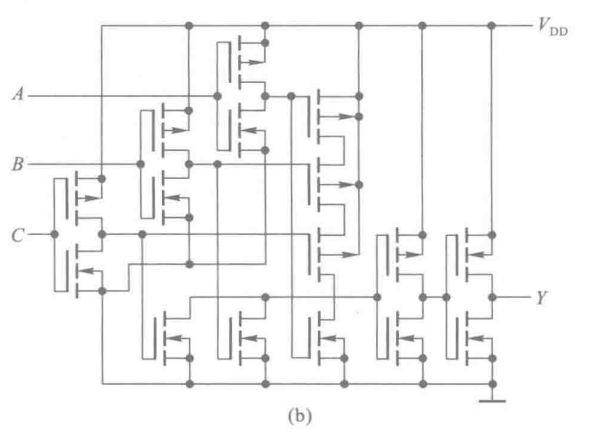
\includegraphics[width=0.6\textwidth]{3.7.b.png}
\end{center}
\textbf{题3.7(b)电路图}

\subsubsection{解答}
该电路为CMOS与或非门结构，PMOS管并联、NMOS管串联的结构实现与或非逻辑。
\begin{itemize}
    \item 逻辑表达式：
\[
Y = \overline{AB + C}
\]
\item 当$AB=1$或$C=1$时，对应NMOS管导通，PMOS管截止，输出低电平；
\item 当$AB=0$且$C=0$时，PMOS管导通，NMOS管截止，输出高电平。
\end{itemize}

\subsection{题3.7(d)：CMOS门电路分析}
\subsubsection{题目}
试分析下图中电路的逻辑功能，写出输出的逻辑函数式。

\begin{center}
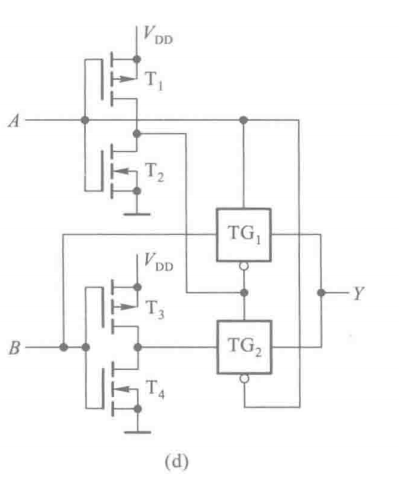
\includegraphics[width=0.5\textwidth]{3.7.d.png}
\end{center}
\textbf{题3.7(d)电路图}

\subsubsection{解答}
该电路由CMOS反相器和传输门组成，是一个二选一数据选择器结构：
\begin{itemize}
    \item 当$B=0$时，传输门$TG_1$导通，$TG_2$截止，$Y = A$；
    \item 当$B=1$时，传输门$TG_2$导通，$TG_1$截止，$Y = \overline{A}$；
    \item 逻辑表达式：
\[
Y = \overline{B}A + B\overline{A} = A \oplus B
\]
\end{itemize}

\subsection{题3.8：输出电压波形分析}
\subsubsection{题目}
试画出下图(a)、(b)两个电路的输出电压波形，输入电压波形如图(c)所示。

\begin{center}
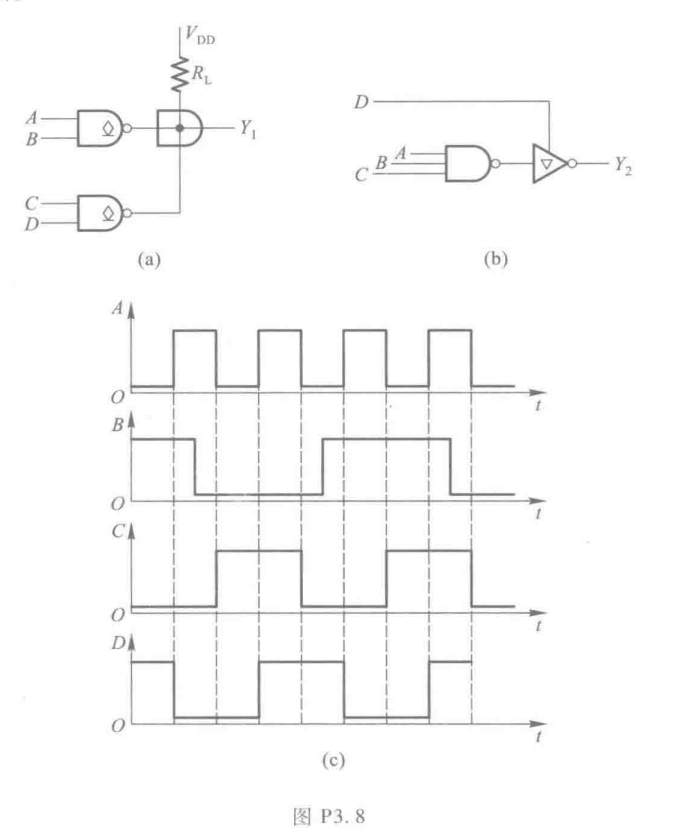
\includegraphics[width=0.7\textwidth]{3.8.png}
\end{center}
\textbf{题3.8电路图与输入波形}

\subsubsection{解答}
\begin{enumerate}
    \item \textbf{电路(a)：OC与非门线与结构}
    \begin{itemize}
        \item 逻辑表达式：$Y_1 = \overline{AB} \cdot \overline{CD} = \overline{AB + CD}$
        \item 输出波形：当$AB=1$或$CD=1$时，输出低电平；否则输出高电平。
    \end{itemize}

    \item \textbf{电路(b)：与非门+三态反相器}
    \begin{itemize}
        \item 逻辑表达式：当使能端$D=1$时，三态门使能，$Y_2 = \overline{ABC}$；当$D=0$时，三态门高阻。
        \item 输出波形：$D=1$时，$Y_2 = \overline{ABC}$；$D=0$时，输出高阻。
    \end{itemize}
\end{enumerate}

% 插入TikZ波形图
\begin{center}
\begin{tikzpicture}[>=stealth,scale=0.85,line width=0.7pt]
    % 时间轴
    \draw[->] (0,0) -- (17,0) node[right] {$t$};
    \foreach \x in {1,3,...,15} \draw (\x,0) -- (\x,-0.3);

    % 信号 A
    \draw (0,2) -- (1,2) -- (1,3) -- (3,3) -- (3,2) -- (5,2) -- (5,3) -- (7,3) -- (7,2) -- (9,2) -- (9,3) -- (11,3) -- (11,2) -- (13,2) -- (13,3) -- (15,3) -- (15,2);
    \node[left] at (0,2.5) {$A$};

    % 信号 B
    \draw (0,4) -- (2,4) -- (2,5) -- (4,5) -- (4,4) -- (6,4) -- (6,5) -- (8,5) -- (8,4) -- (10,4) -- (10,5) -- (12,5) -- (12,4) -- (14,4) -- (14,5) -- (16,5) -- (16,4);
    \node[left] at (0,4.5) {$B$};

    % 信号 C
    \draw (0,6) -- (4,6) -- (4,7) -- (8,7) -- (8,6) -- (12,6) -- (12,7) -- (16,7) -- (16,6);
    \node[left] at (0,6.5) {$C$};

    % 信号 D
    \draw (0,8) -- (2,8) -- (2,9) -- (6,9) -- (6,8) -- (10,8) -- (10,9) -- (14,9) -- (14,8);
    \node[left] at (0,8.5) {$D$};

    % 输出 Y1 (线与)
    \draw[red, thick]
    (0,10) -- (2,10)
    -- (2,9)  -- (4,9)
    -- (4,10) -- (6,10)
    -- (6,9)  -- (8,9)
    -- (8,10) -- (10,10)
    -- (10,9) -- (12,9)
    -- (12,10) -- (16,10);
    \node[left, red] at (0,9.5) {$Y_1$};

    % 输出 Y2 (三态)
    \draw[blue, thick]
    (0,12) -- (2,12)
    -- (2,11.5) -- (6,11.5) node[midway, fill=white] {高阻}
    -- (6,12) -- (8,12)
    -- (8,11.5) -- (12,11.5) node[midway, fill=white] {高阻}
    -- (12,12) -- (14,12)
    -- (14,11.5) -- (16,11.5);
    \node[left, blue] at (0,11.5) {$Y_2$};
\end{tikzpicture}
\end{center}

\subsection{题3.12：CMOS门电路输出电平判断}
\subsubsection{题目}
说明图中各门电路的输出是高电平还是低电平。已知它们都是74HC系列的CMOS电路。

\begin{center}
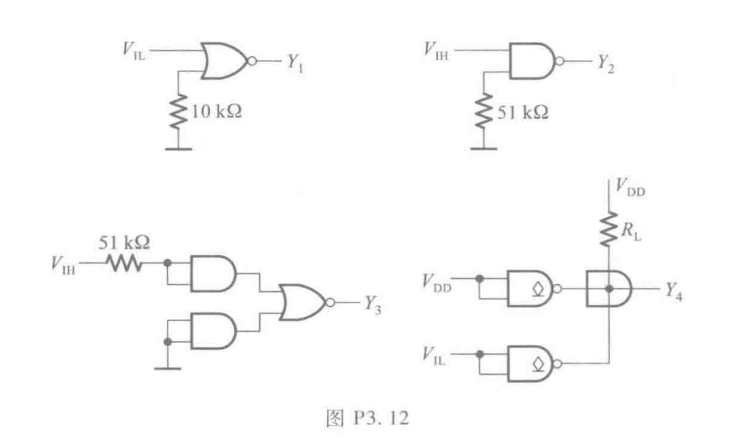
\includegraphics[width=0.6\textwidth]{3.12.png}
\end{center}
\textbf{题3.12电路图}

\subsubsection{解答}
CMOS电路输入阻抗极高，输入通过电阻接地时，电阻上无电流，输入端电位为0V；接高电平通过电阻时，输入端电位为高电平。
\begin{enumerate}
    \item $Y_1$：或非门，输入为$V_{IL}$和$0V$（通过10k$\Omega$电阻接地），$Y_1 = \overline{V_{IL} + 0} = \overline{0} = 1$（高电平）。
    \item $Y_2$：与非门，输入为$V_{IH}$和$0V$（通过51k$\Omega$电阻接地），$Y_2 = \overline{V_{IH} \cdot 0} = \overline{0} = 1$（高电平）。
    \item $Y_3$：两个与非门输入分别为$V_{IH}$和0、1，输出为$\overline{V_{IH} \cdot 0} = 1$和$\overline{1 \cdot 1} = 0$，再经或非门，$Y_3 = \overline{1 + 0} = 0$（低电平）。
    \item $Y_4$：两个OC门线与，输入分别为$V_{DD}$和$V_{IL}$，输出为$\overline{V_{DD} \cdot V_{DD}} = 0$和$\overline{V_{IL} \cdot V_{IL}} = 1$，线与后$Y_4 = 0 \cdot 1 = 0$（低电平）。
\end{enumerate}

\subsection{题3.13：TTL与非门输入电压测量}
\subsubsection{题目}
试说明在下列情况下，用万用表测量下图中的$v_{I2}$端得到的电压各为多少：
\begin{enumerate}
    \item $v_{I1}$悬空；
    \item $v_{I1}$接低电平(0.2V)；
    \item $v_{I1}$接高电平(3.2V)；
    \item $v_{I1}$经51$\Omega$电阻接地；
    \item $v_{I1}$经10k$\Omega$电阻接地。
\end{enumerate}
图中的与非门为74系列的TTL电路，万用表使用5V量程，内阻为20k$\Omega$/V。

\begin{center}
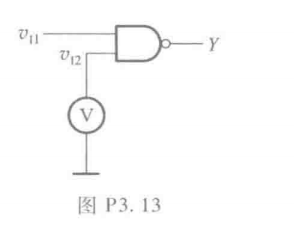
\includegraphics[width=0.3\textwidth]{3.13.png}
\end{center}
\textbf{题3.13电路图}

\subsubsection{解答}
TTL与非门输入级为多发射极三极管，输入特性存在开门/关门电平：
\begin{enumerate}
    \item $v_{I1}$悬空：相当于输入高电平，三极管导通，$v_{I2} \approx 1.4V$（PN结压降之和）。
    \item $v_{I1}=0.2V$：三极管基极电位被钳位，$v_{I2} = 0.2V + 0.7V = 0.9V$。
    \item $v_{I1}=3.2V$：三极管导通，$v_{I2} \approx 1.4V$。
    \item $v_{I1}$经51$\Omega$接地：输入电流在电阻上压降小，$v_{I1}$等效低电平，$v_{I2} \approx 0.9V$。
    \item $v_{I1}$经10k$\Omega$接地：电阻大于开门电阻，$v_{I1}$等效高电平，$v_{I2} \approx 1.4V$。
\end{enumerate}

\subsection{题3.17：TTL或非门扇出数计算}
\subsubsection{题目}
在下图所示由74系列或非门组成的电路中，试求门$G_M$能驱动多少同样的或非门。要求$G_M$输出的高、低电平满足$V_{OH} \ge 3.2V, V_{OL} \le 0.4V$。或非门每个输入端的输入电流为$I_{IL} \le -1.6mA, I_{IH} \le 40\mu A$。$V_{OL} \le 0.4V$时输出电流的最大值为$I_{OL(max)} = 16mA$，$V_{OH} \ge 3.2V$时输出电流的最大值为$I_{OH(max)} = -0.4mA$。$G_M$的输出电阻可忽略不计。

\begin{center}
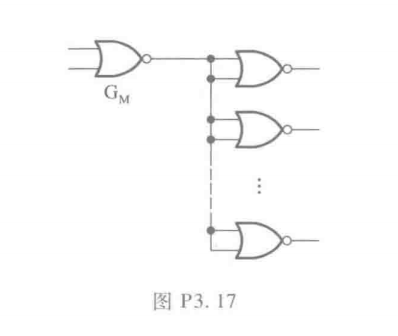
\includegraphics[width=0.4\textwidth]{3.17.png}
\end{center}
\textbf{题3.17电路图}

\subsubsection{解答}
扇出数由低电平驱动能力和高电平驱动能力的最小值决定：
\begin{enumerate}
    \item \textbf{低电平扇出数$N_L$}：

每个负载或非门有2个输入端，低电平输入电流为$|I_{IL}|=1.6mA$，总电流为$N \times 2 \times 1.6mA$，需满足：
\[
N_L \times 2 \times 1.6mA \le I_{OL(max)} = 16mA \implies N_L \le 5
\]

    \item \textbf{高电平扇出数$N_H$}：

每个负载或非门有2个输入端，高电平输入电流为$I_{IH}=40\mu A$，总电流为$N \times 2 \times 40\mu A$，需满足：
\[
N_H \times 2 \times 40\mu A \le |I_{OH(max)}| = 0.4mA \implies N_H \le 5
\]
\end{enumerate}

最终扇出数取最小值：
\[
N = \min(N_L, N_H) = 5
\]

\subsection{题3.23：OC门驱动三极管电路分析}
\subsubsection{题目}
在下图(a)所示电路中已知三极管导通时$V_{BE}=0.7V$，饱和压降$V_{CE(sat)}=0.3V$，饱和导通内阻为$R_{CE(sat)}=20\Omega$，三极管的电流放大系数$\beta=100$。OC门$G_1$输出截止时的漏电流约为50$\mu$A，导通时允许的最大负载电流为16mA，输出低电平$\le 0.3V$。$G_2 \sim G_5$均为74系列TTL电路，其中$G_2$为反相器，$G_3$和$G_4$是与非门，$G_5$是或非门，它们的输入特性如图(b)所示。试问：
\begin{enumerate}
    \item 在三极管集电极输出的高、低电压满足$V_{OH} \ge 3.5V, V_{OL} \le 0.3V$的条件下，$R_B$的取值范围有多大？
    \item 若将OC门改成推挽式输出的TTL门电路，会发生什么问题？
\end{enumerate}

\begin{center}
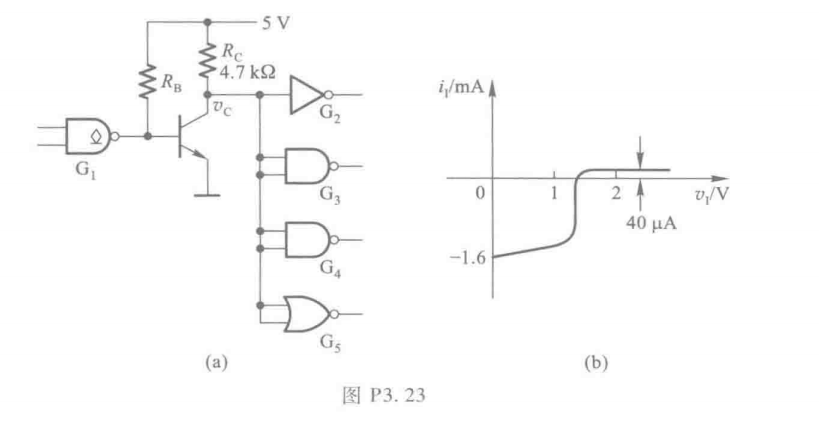
\includegraphics[width=0.7\textwidth]{3.23.png}
\end{center}
\textbf{题3.23电路图与输入特性}

\subsubsection{解答}
\paragraph{(1) $R_B$取值范围计算}
\begin{itemize}
    \item \textbf{三极管饱和导通条件}：基极电流$I_B \ge I_{BS} = \dfrac{I_{CS}}{\beta}$

$I_{CS} = \dfrac{V_{CC} - V_{CE(sat)}}{R_C} + 4|I_{IL}|$（4个负载门的低电平输入电流）

代入数据：
$I_{CS} = \dfrac{5-0.3}{4.7k\Omega} + 4 \times 1.6mA \approx 1mA + 6.4mA = 7.4mA$

$I_{BS} = 7.4mA / 100 = 74\mu A$

基极电流由OC门导通时提供：
$I_B = \dfrac{V_{CC} - V_{BE} - V_{OL}}{R_B} \ge I_{BS}$

解得：
$R_B \le \dfrac{5-0.7-0.3}{74\mu A} \approx 54k\Omega$

    \item \textbf{三极管截止条件}：OC门截止时，漏电流$I_{OH}=50\mu A$，基极电位$V_B \le 0$，即：
$I_{OH} \times R_B \le V_{BE} \implies R_B \le \dfrac{0.7V}{50\mu A} = 14k\Omega$

同时OC门导通时负载电流不超过最大值：
$\dfrac{5-0.7-0.3}{R_B} \le 16mA \implies R_B \ge \dfrac{4V}{16mA} = 250\Omega$
\end{itemize}

综合得：
\[
250\Omega \le R_B \le 14k\Omega
\]

\paragraph{(2) 推挽式TTL门的问题}
推挽式输出的TTL门无法承受OC门的线与特性，当输出为低电平时，三极管基极电流会灌入TTL门的输出级，导致输出管过流损坏；且推挽输出无法实现线与逻辑，不能直接驱动三极管基极。